\section{Séance 9}

\paragraph{1. } Donnez une autre représentation planaire du graphe suivant où la face spécifiée (egf) devient la face extérieure.

\begin{figure}[h!]
  \begin{center}
    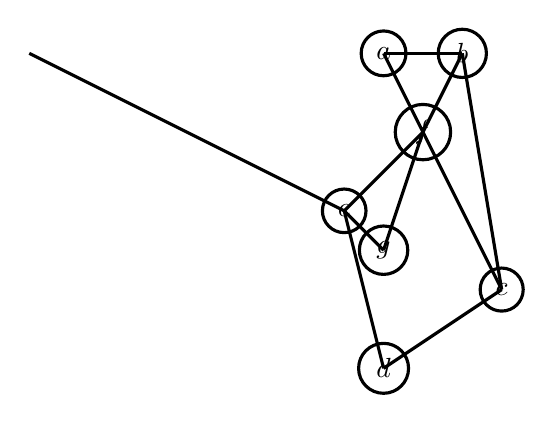
\begin{tikzpicture}[scale=1,looseness=1,auto,line width=.4mm]
      \path (-.5, 2) node[draw,shape=circle] (1)  {$a$};
      \path (.5, 2)  node[draw,shape=circle] (2)  {$b$};
      \path (1,-1) node[draw,shape=circle] (3)  {$c$};
      \path ( -.5, -2) node[draw,shape=circle] (6)  {$d$};
      \path ( -1, 0) node[draw,shape=circle] (5)  {$e$};
      \path (  0, 1) node[draw,shape=circle] (4)  {$f$};
      \path (  -.5, -.5) node[draw,shape=circle] (7)  {$g$};

       \draw (-1, 0) -- ( -.5,-2); %ed
      \draw (-1, 0) -- ( -.5,-.5); %eg
      \draw (-1, 0) -- ( 0,1); %ef
      \draw (-1, 0) -- ( -5,2); %ea
      \draw (-.5, -2) -- ( 1,-1); %dc
      \draw ( -.5, -.5) -- (0,1); %gf
      \draw ( -.5, 2) -- ( 0,1); %af
      \draw ( -.5, 2) -- (.5,2); %ab
      \draw ( 0, 1) -- ( .5,2); %fb
      \draw ( 0, 1) -- ( 1,-1); %fc
      \draw ( .5, 2) -- ( 1,-1); %bc

    \end{tikzpicture}
  \end{center}
\end{figure}

\paragraph{2. } Un graphe planaire peut-il être représenté sur un cylindre bi-infini sans ses arêtes ne se croisent? La réciproque est-elle vraie?  Et pour un graphe sur un tore?

\paragraph{3. } Les graphes suivants sont-ils planaires? 

\begin{figure}[h!]
  \begin{center}
   \begin{tabular}{lcccr}
    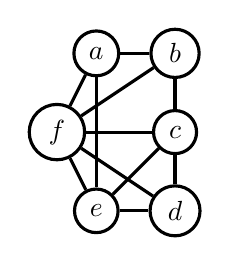
\begin{tikzpicture}[scale=1,looseness=1,auto,line width=.4mm]

      \path (0,2) node[draw,shape=circle] (1)  {$a$};
      \path (1,2) node[draw,shape=circle] (2)  {$b$};
      \path (1,1) node[draw,shape=circle] (3)  {$c$};
      \path (1,0) node[draw,shape=circle] (4)  {$d$};
      \path (0,0) node[draw,shape=circle] (5)  {$e$};
      \path (-.5,1) node[draw,shape=circle] (6)  {$f$};

      \draw (1)  -- (2);
      \draw (1)  -- (5) ; 
      \draw (1)  -- (6)  ;
      \draw (2)  -- (3)  ;
      \draw (2)  -- (6)  ;
      \draw (3)  -- (6)  ;
      \draw (3) -- (4) ;
      \draw (3) -- (5) ;
      \draw (4) -- (6) ;
      \draw (4)  -- (5) ;
      \draw (5)  -- (6)  ;
   \end{tikzpicture}

 & \hspace{1cm} &
      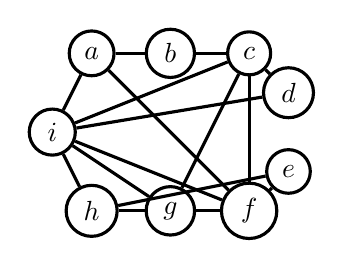
\begin{tikzpicture}[scale=1,looseness=1,auto,line width=.4mm]
   
     \path (-1,1) node[draw,shape=circle] (1)  {$a$};
      \path (0,1) node[draw,shape=circle] (2)  {$b$};
      \path (1,1) node[draw,shape=circle] (3)  {$c$};
      \path (1.5,.5) node[draw,shape=circle] (4)  {$d$};
      \path (1.5,-.5) node[draw,shape=circle] (5)  {$e$};
      \path (1,-1) node[draw,shape=circle] (6)  {$f$};
      \path (0,-1) node[draw,shape=circle] (7)  {$g$};
      \path (-1,-1) node[draw,shape=circle] (8)  {$h$};
      \path (-1.5,0) node[draw,shape=circle] (9)  {$i$};

      \draw (1)  -- (2);
      \draw (1)  -- (6) ; 
      \draw (1)  -- (9)  ;
      \draw (2)  -- (3)  ;
      \draw (3)  -- (4)  ;
      \draw (3)  -- (6)  ;
      \draw (3) -- (7) ;
      \draw (3) -- (9) ;
      \draw (4) -- (9) ;
      \draw (5)  -- (6) ;
      \draw (5)  -- (8)  ;
       \draw (6)  -- (7)  ;
      \draw (6) -- (9) ;
      \draw (7) -- (8) ;
      \draw (7) -- (9) ;
      \draw (8)  -- (9) ;
      
   \end{tikzpicture}

& \hspace{1cm} &
      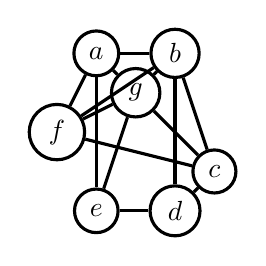
\begin{tikzpicture}[scale=1,looseness=1,auto,line width=.4mm]
   
     \path (-.5,1) node[draw,shape=circle] (1)  {$a$};
      \path (.5,1) node[draw,shape=circle] (2)  {$b$};
      \path (1,-.5) node[draw,shape=circle] (3)  {$c$};
      \path (.5,-1) node[draw,shape=circle] (4)  {$d$};
      \path (-.5,-1) node[draw,shape=circle] (5)  {$e$};
      \path (-1,0) node[draw,shape=circle] (6)  {$f$};
      \path (0,.5) node[draw,shape=circle] (7)  {$g$};

      \draw (1)  -- (2);
      \draw (1)  -- (6) ; 
      \draw (1)  -- (5)  ;
      \draw (1)  -- (7)  ;
      \draw (2)  -- (3)  ;
      \draw (2)  -- (4)  ;
      \draw (2) -- (7) ;
      \draw (2) -- (6) ;
      \draw (3) -- (4) ;
      \draw (3)  -- (6) ;
      \draw (3)  -- (7)  ;
       \draw (4)  -- (5)  ;
      \draw (5) -- (7) ;
      \draw (6) -- (7) ;
      
   \end{tikzpicture}

\end{tabular}
 \end{center}
\end{figure}

\paragraph{4. } Supposez qu’un graphe connexe planaire a 6 sommets, chacun de degré 4. En combien de régions le plan est-il divisé par une représentation planaire de ce graphe?

\paragraph{5. } Le complémentaire $\bar{G}$ d’un graphe $G = (V,E)$ de $n$ sommets est donné par $\bar{G} = (V, E(K_n) - E)$. Montrez que si $n \geq 11$, au moins un des deux graphes $G$ ou $\bar{G}$ n’est pas planaire.

\paragraph{6. } Sous quelle condition est-il possible d’ajouter une arête à un graphe planaire en conservant la planarité? Déduisez le nombre total d’arêtes qu’il est possible d’ajouter à un graphe planaire de $n$ sommets et $m$ arêtes tout en conservant la planarité.

\paragraph{7. } Soit un graphe $G$ 3-régulier tel que tout sommet est incident à une face de degré 4, une face de degré 6 et une face de degré 8. Sans dessiner $G$, déterminez le nombre de faces de $G$. 

\paragraph{8. }Montrez que si tous les sommets d’un graphe planaire $G$ sont de degré pair, alors toutes les faces de $G$ peuvent être coloriées en deux couleurs de telle sorte que deux faces adjacentes n’aient jamais la même couleur.

\paragraph{9. } Un circuit électrique connecte des terminaux de deux types $A$ et $B$. Chaque terminal $A$ est connecté à chaque terminal $B$. Montrez qu’un tel circuit peut être imprimé sur les deux faces d’une seule feuille isolante si les terminaux traversent la feuille.
